\documentclass[utf8]{article} % for all articles
\usepackage{url,hyperref,lineno,microtype}
\usepackage[onehalfspacing]{setspace}
\usepackage{cleveref}
\usepackage{physics}
\usepackage{siunitx}
\usepackage{xr}

% \graphicspath{{../figures/}}

\begin{document}
\firstpage{1}

\title{Response}
\maketitle

% TODO: Add line numbers everywhere.
\section{Major comments Reviewer 1}
\textbf{On n-n notation.} As suggested by the reviewer, we've changed the notation from $n-n$ to $n:n$ to denote the type of burst solution.

\section{Minor comments Reviewer 1}

\subsection{Changes to the nullclines plot}
In order to reduce the number of figures we have merged figures 1 and 5, and adjusted added a paragraph describing the non-zero constant synaptic conductance case at the end of the methods part.

\section{Release delay}
Due to the changes to the single cell model parameters, i.e. reducing the applied current from $I=6 \si{\mu A/cm^{2}}$ to $I=3.8\si{\mu A/cm^{2}}$, the $v$-nullcline moved down along the $w$-nullcline.
% I've checked that old HB value manually, should be correct.
This made the system become more excitable, that is the subcritical Andronov-Hopf bifurcation point where the fixed point changes stability moved from $\bar g=0.038$ to $\bar g=0.0038$.
As a consequence, the release delay seen previously is now negligible for all $n:n$ solutions, see figure \cref{fig:release-delay}.

\begin{figure}[h!]
  \centering
  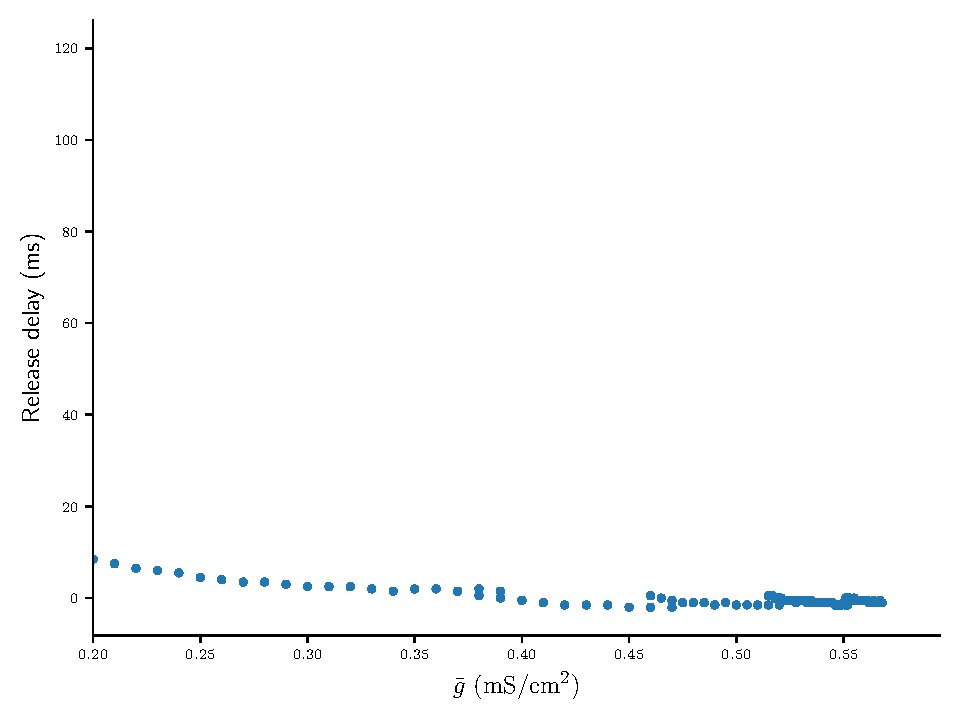
\includegraphics[width=0.8\textwidth]{release-delay.pdf}
  \caption{Numerically computed graph of the release delay as a function of $\bar g$~\label{fig:release-delay}}
\end{figure}


\bibliographystyle{frontiersinHLTH&FPHY} % for Health, Physics and Mathematics articles
\bibliography{bibliography.bib}

\end{document}

%%% Local Variables:
%%% mode: latex
%%% TeX-master: t
%%% End:
